%==============================================================================
% Figure: Casimir Cavity Geometries for ZPE Harvesting
% Source: Chapter 28 (Energy Technologies)
% Purpose: Illustrate three common resonant cavity configurations
%==============================================================================
\begin{figure}[htbp]
  \centering
  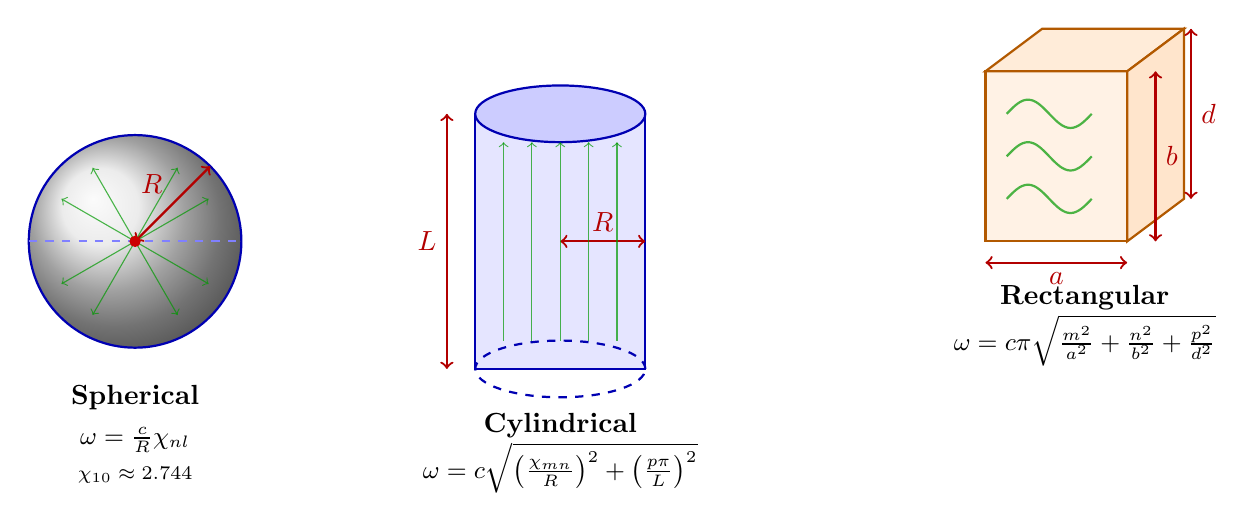
\begin{tikzpicture}[scale=0.9]

    % ====== SPHERICAL CAVITY ======
    \begin{scope}[xshift=-6cm]
      % Outer sphere
      \shade[ball color=gray!20] (0,0) circle (1.5cm);
      \draw[thick, blue!70!black] (0,0) circle (1.5cm);

      % Cross-section line
      \draw[thick, dashed, blue!50] (-1.5,0) -- (1.5,0);

      % Radius annotation
      \draw[<->, red!70!black, thick] (0,0) -- (1.06,1.06) node[midway, above left] {$R$};

      % Field lines (radial)
      \foreach \angle in {30,60,120,150,210,240,300,330} {
        \draw[->, green!60!black, opacity=0.7]
          (0,0) -- ({1.2*cos(\angle)},{1.2*sin(\angle)});
      }

      % Center point
      \fill[red!80!black] (0,0) circle (0.08cm);

      % Title and resonance formula
      \node[font=\bfseries] at (0,-2.2) {Spherical};
      \node[font=\small, align=center] at (0,-2.8) {$\omega = \frac{c}{R}\chi_{nl}$};
      \node[font=\scriptsize, align=center] at (0,-3.3) {$\chi_{10} \approx 2.744$};
    \end{scope}

    % ====== CYLINDRICAL CAVITY ======
    \begin{scope}[xshift=0cm]
      % Cylinder body
      \fill[blue!10!white, draw=blue!70!black, thick]
        (-1.2,-1.8) rectangle (1.2,1.8);

      % Top ellipse
      \fill[blue!20!white, draw=blue!70!black, thick]
        (0,1.8) ellipse (1.2cm and 0.4cm);

      % Bottom ellipse (back)
      \draw[blue!70!black, thick, dashed]
        (0,-1.8) ellipse (1.2cm and 0.4cm);

      % Dimensions
      \draw[<->, red!70!black, thick] (-1.6,-1.8) -- (-1.6,1.8)
        node[midway, left] {$L$};
      \draw[<->, red!70!black, thick] (0,0) -- (1.2,0)
        node[midway, above] {$R$};

      % Field lines (vertical)
      \foreach \x in {-0.8,-0.4,0,0.4,0.8} {
        \draw[->, green!60!black, opacity=0.7] (\x,-1.4) -- (\x,1.4);
      }

      % Title and resonance formula
      \node[font=\bfseries] at (0,-2.6) {Cylindrical};
      \node[font=\small, align=center] at (0,-3.2)
        {$\omega = c\sqrt{\left(\frac{\chi_{mn}}{R}\right)^2 + \left(\frac{p\pi}{L}\right)^2}$};
    \end{scope}

    % ====== RECTANGULAR CAVITY ======
    \begin{scope}[xshift=6cm]
      % 3D rectangular box (isometric view)
      \fill[orange!10!white, draw=orange!70!black, thick]
        (0,0) -- (2,0) -- (2,2.4) -- (0,2.4) -- cycle;
      \fill[orange!15!white, draw=orange!70!black, thick]
        (0,2.4) -- (0.8,3) -- (2.8,3) -- (2,2.4) -- cycle;
      \fill[orange!20!white, draw=orange!70!black, thick]
        (2,0) -- (2.8,0.6) -- (2.8,3) -- (2,2.4) -- cycle;

      % Dimensions
      \draw[<->, red!70!black, thick] (0,-0.3) -- (2,-0.3)
        node[midway, below] {$a$};
      \draw[<->, red!70!black, thick] (2.4,0) -- (2.4,2.4)
        node[midway, right] {$b$};
      \draw[<->, red!70!black, thick] (2.9,0.6) -- (2.9,3)
        node[midway, right] {$d$};

      % Field pattern (standing wave)
      \foreach \y in {0.6,1.2,1.8} {
        \draw[green!60!black, thick, opacity=0.7]
          (0.3,\y) sin (0.6,\y+0.2) cos (0.9,\y) sin (1.2,\y-0.2) cos (1.5,\y);
      }

      % Title and resonance formula
      \node[font=\bfseries] at (1.4,-0.8) {Rectangular};
      \node[font=\small, align=center] at (1.4,-1.4)
        {$\omega = c\pi\sqrt{\frac{m^2}{a^2} + \frac{n^2}{b^2} + \frac{p^2}{d^2}}$};
    \end{scope}

  \end{tikzpicture}

  \caption{Three common resonant cavity geometries for Zero-Point Energy (ZPE) harvesting. \textbf{Left:} Spherical cavity with radius $R$, supporting spherical Bessel modes with zeros $\chi_{nl}$. Radial field lines (green) show TE/TM mode patterns. \textbf{Center:} Cylindrical cavity with radius $R$ and length $L$, supporting Bessel function modes $J_m$ with zeros $\chi_{mn}$. \textbf{Right:} Rectangular cavity with dimensions $a \times b \times d$, supporting integer mode numbers $(m,n,p)$. Resonance formulas show dimensional scaling: frequency $\omega \propto 1/R$ (spherical/cylindrical) or $\omega \propto 1/\sqrt{a^2 + b^2 + d^2}$ (rectangular). All assume vacuum permittivity $\epsilon_r = \mu_r = 1$; material-filled cavities multiply by $\sqrt{\epsilon_r \mu_r}$.}
  \label{fig:ch28:cavity_geometries}
\end{figure}
%==============================================================================
